\documentclass{beamer}
\usepackage{relsize}
\usepackage{color}

\usepackage{listings}
\usetheme{CambridgeUS}
%\usepackage{beamerthemesplit} % new
\usepackage{enumitem}
\usepackage{amsmath}                    % See geometry.pdf to learn the layout options.
\usepackage{amsthm}                   % See geometry.pdf to learn the layout options. There
\usepackage{amssymb}                    % See geometry.pdf to learn the layout options.
\usepackage[utf8]{inputenc}
\usepackage{graphicx}
\usepackage[english,bulgarian]{babel}

\usepackage{caption}
\usepackage{tikz}

\usetheme{CambridgeUS}
\usecolortheme{crane}

\lstset{language=C++,
                basicstyle=\ttfamily,
                keywordstyle=\color{blue}\ttfamily,
                stringstyle=\color{red}\ttfamily,
                commentstyle=\color{green}\ttfamily,
                morecomment=[l][\color{magenta}]{\#}
}

\newtheorem{mydef}{Дефиниция}[section]
\newtheorem{lem}{Лема}[section]
\newtheorem{thm}{Твърдение}[section]

\DeclareMathOperator{\restrict}{\upharpoonright}

\setitemize{label=\usebeamerfont*{itemize item}%
  \usebeamercolor[fg]{itemize item}
  \usebeamertemplate{itemize item}}

\setbeamercovered{transparent}

\captionsetup{font=tiny} 

\begin{document}
\title[Увод в курса]{Функции от по-висок ред}
\frame{\titlepage}

\section{Функции от по-висок ред}
\subsection{}

\begin{frame}
  \centerline{Функциите като параметри на други функции}
\end{frame}

\begin{frame}[fragile]
  \frametitle{filter}

  \begin{itemize}
    \item Прости примери (>, even)
    \item Примери: структурирани данни
    \item Примери: операции над множества
    \item Примери: номериране с \verb#zip#
    \item quicksort
  \end{itemize}

\end{frame}

\begin{frame}[fragile]
  \frametitle{По-задълбочен поглед}

  \begin{itemize}
    \item Реализация на $filter$
    \item Производителност
    \item Филтриране на безкрайни списъци
  \end{itemize}

  \begin{tikzpicture}[remember picture,overlay]
    \node[xshift=5mm,yshift=-15mm,anchor=north west] at (current page.north west){%
    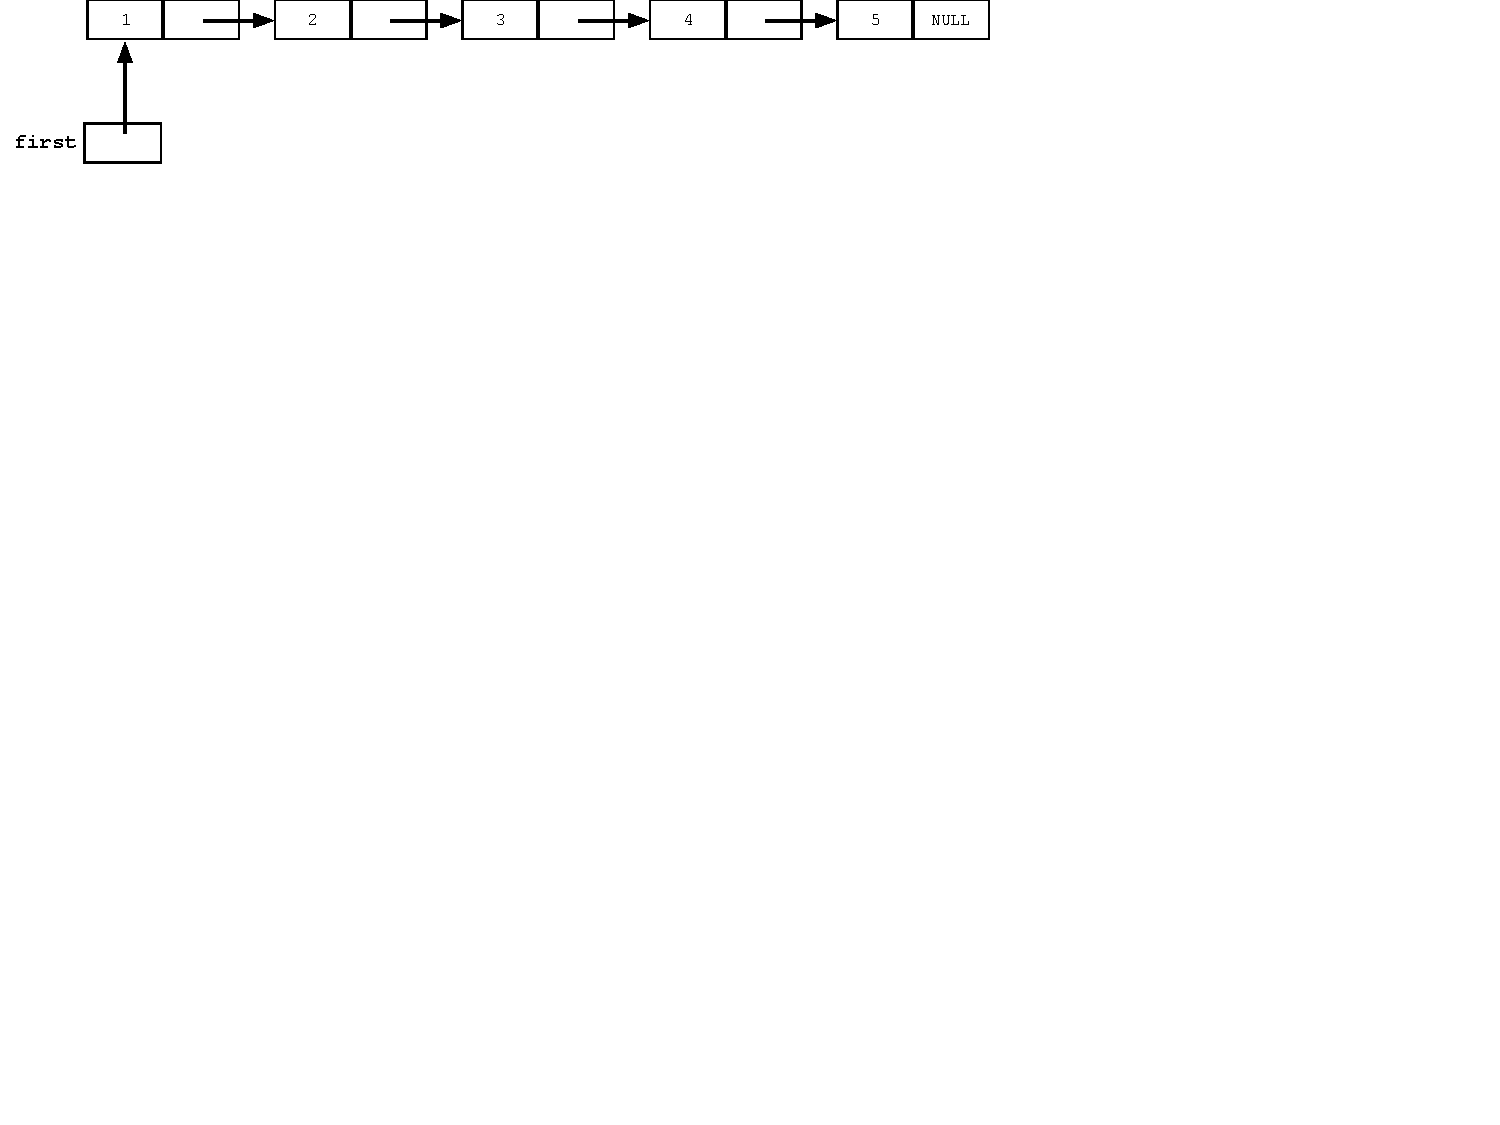
\includegraphics[width=155mm]{images/02_ll_flatchain.pdf}};
  \end{tikzpicture}
  
\end{frame}

\begin{frame}[fragile]
  \frametitle{map}

  \begin{itemize}
    \item Прости примери (+1, even, digits, toUpper)
    \item Примери: структурирани данни
    \item Списъци от функции
    \item Реализация
  \end{itemize}

\end{frame}

\begin{frame}[fragile]
  \frametitle{foldr}

  \begin{itemize}
    \item Прилагане на опреация с акумулатор
    \item Примери: сума, произведение, конкатенация
    \item $map$ и $filter$ с $foldr$
    \item $elem$ с $foldr$. Сравнение с $elem$
    \item Примери: структурирани данни
    \item Реализация
  \end{itemize}

\end{frame}


\begin{frame}[fragile]
  \frametitle{foldl}

  \begin{itemize}
    \item Реализация
    \item $reverse$ с $foldl$
  \end{itemize}
\end{frame}

\begin{frame}[fragile]
  \frametitle{foldl1, foldr1}

  \begin{itemize}
    \item maximum, minimum
  \end{itemize}
\end{frame}


\begin{frame}
  \centerline{MapReduce}
\end{frame}


\begin{frame}[fragile]
  \frametitle{MapReduce}

  \begin{tikzpicture}[remember picture,overlay]
    \node[xshift=00mm,yshift=-15mm,anchor=north] at (current page.north){%
    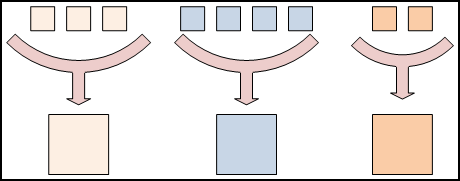
\includegraphics[width=55mm]{images/mapreduce}};
  \end{tikzpicture}


  \begin{itemize}
    \item Пример със структурирани данни
    \item ``Език'' за заявки
  \end{itemize}

\end{frame}


\begin{frame}[fragile]
  \frametitle{Други примери}

  zipwith, takewhile, dropwhile, iterate, unfoldr

\end{frame}


\begin{frame}[fragile]
  \frametitle{Път в лабиринт}

  \begin{lstlisting}[basicstyle=\tiny,language=Haskell]
--findGold :: game visited -> path
findGold :: Maybe Game -> [Pos] -> [Pos]
findGold Nothing _ = []
findGold (Just g@(Game p w)) visited
    | foundGold g = [p]
    | (stuck g) || (elem p visited) = []
    | downpath /= [] = p : downpath
    | rightpath /= [] = p : rightpath
    | uppath /= [] = p : uppath
    | leftpath /= [] = p : leftpath
    where downpath = findGold (down g) (p:visited)
          rightpath = findGold (right g) (p:visited)
          uppath = findGold (up g) (p:visited)
          leftpath = findGold (left g) (p:visited)  
  \end{lstlisting}
  
\end{frame}


\begin{frame}[fragile]
  \frametitle{mapMaybe}

\begin{lstlisting}[basicstyle=\tiny,language=Haskell]
findGold :: Maybe Game -> [Pos] -> Maybe [Pos]
findGold Nothing _ = Nothing
findGold (Just g@(Game p w)) visited
    | foundGold g = Just [p]
    | (stuck g) || (elem p visited) || null routes = Nothing
    | otherwise = Just $ p : (head routes)
    where routes = mapMaybe (\dir -> findGold (dir g) (p:visited))
                            [down, right, up, left]  
\end{lstlisting}
  
\end{frame}

\begin{frame}[fragile]
  \frametitle{без Lambda}

\begin{lstlisting}[basicstyle=\tiny,language=Haskell]
findGold :: Maybe Game -> [Pos] -> Maybe [Pos]
findGold Nothing _ = Nothing
findGold (Just g@(Game p w)) visited
    | foundGold g = Just [p]
    | (stuck g) || (elem p visited) || null routes = Nothing
    | otherwise = Just $ p : (head routes)
    where routes = mapMaybe ((flip findGold) (p:visited))
                            [down g, right g, up g, left g]  
\end{lstlisting}
  
\end{frame}

\begin{frame}
  \centerline{List Comprehensions}
\end{frame}

\begin{frame}[fragile]
  \frametitle{List Comprehensions}

\verb#map# и \verb#filter# в едно

\bigskip

\begin{lstlisting}[basicstyle=\small,language=Haskell]
squares = [x*x | x <- [1..10]]
evens = [x | x <- [1..10], even x]
squaresOfEvens = [x*x | x <- [1..10], even x]
\end{lstlisting}
  
\bigskip

Прилича ли на $\{x^2 | x \in \{1,2,\dots,10\} \land x \equiv 0 (mod 2)\}$?
\end{frame}


\begin{frame}[fragile]
  \frametitle{List Comprehensions}

Какво става ако комбинираме повече от един списък?

\bigskip

\begin{lstlisting}[basicstyle=\small,language=Haskell]
pairs = [(x,y) | x <- [1..10], y <- [1..10]]
\end{lstlisting}
  
\bigskip

Прилича ли на $\{x^2 | x \in \{1,2,\dots,10\} \land x \equiv 0 (mod 2)\}$?
\end{frame}

\begin{frame}[fragile]
  \frametitle{List Comprehensions}

Работа с безкрайни списъци

\bigskip

\begin{lstlisting}[basicstyle=\small,language=Haskell]
squares = [x*x | x <- [1..]]
\end{lstlisting}
  
\end{frame}

\begin{frame}[fragile]
  \frametitle{List Comprehensions}

Трябва да се внимава

\bigskip

\begin{lstlisting}[basicstyle=\small,language=Haskell]
allpairs = [(x,y) | x <- [1..], y <- [1..]]
take 10 allpairs
\end{lstlisting}
  
\bigskip

А така?

\begin{lstlisting}[basicstyle=\small,language=Haskell]
allpairs = [(x,y) | x <- [1..], x <= 10, y <- [1..]]
take 10 allpairs
\end{lstlisting}

\end{frame}  

\begin{frame}
  \centerline{Функции, които връщат функции. Closures}
\end{frame}

\begin{frame}[fragile]
  \frametitle{Операции с финкции}

\begin{itemize}
  \item С функциите работим като с данни: прилагаме операции над тях
  \item Какви операции знаем над функции?
\end{itemize}

\bigskip

\begin{itemize}
  \item Прилагане на функция. Currying
  \item Композиция (., >>=)
  \item Елементи на списъци и n-торки
  \item Дефиниране
  \item Дефиниране с $\lambda$
\end{itemize}

\end{frame}


\begin{frame}[fragile]
  \frametitle{Closures}
  \begin{tikzpicture}[remember picture,overlay]
    \node[xshift=0,yshift=-14mm,anchor=north] at (current page.north){%
    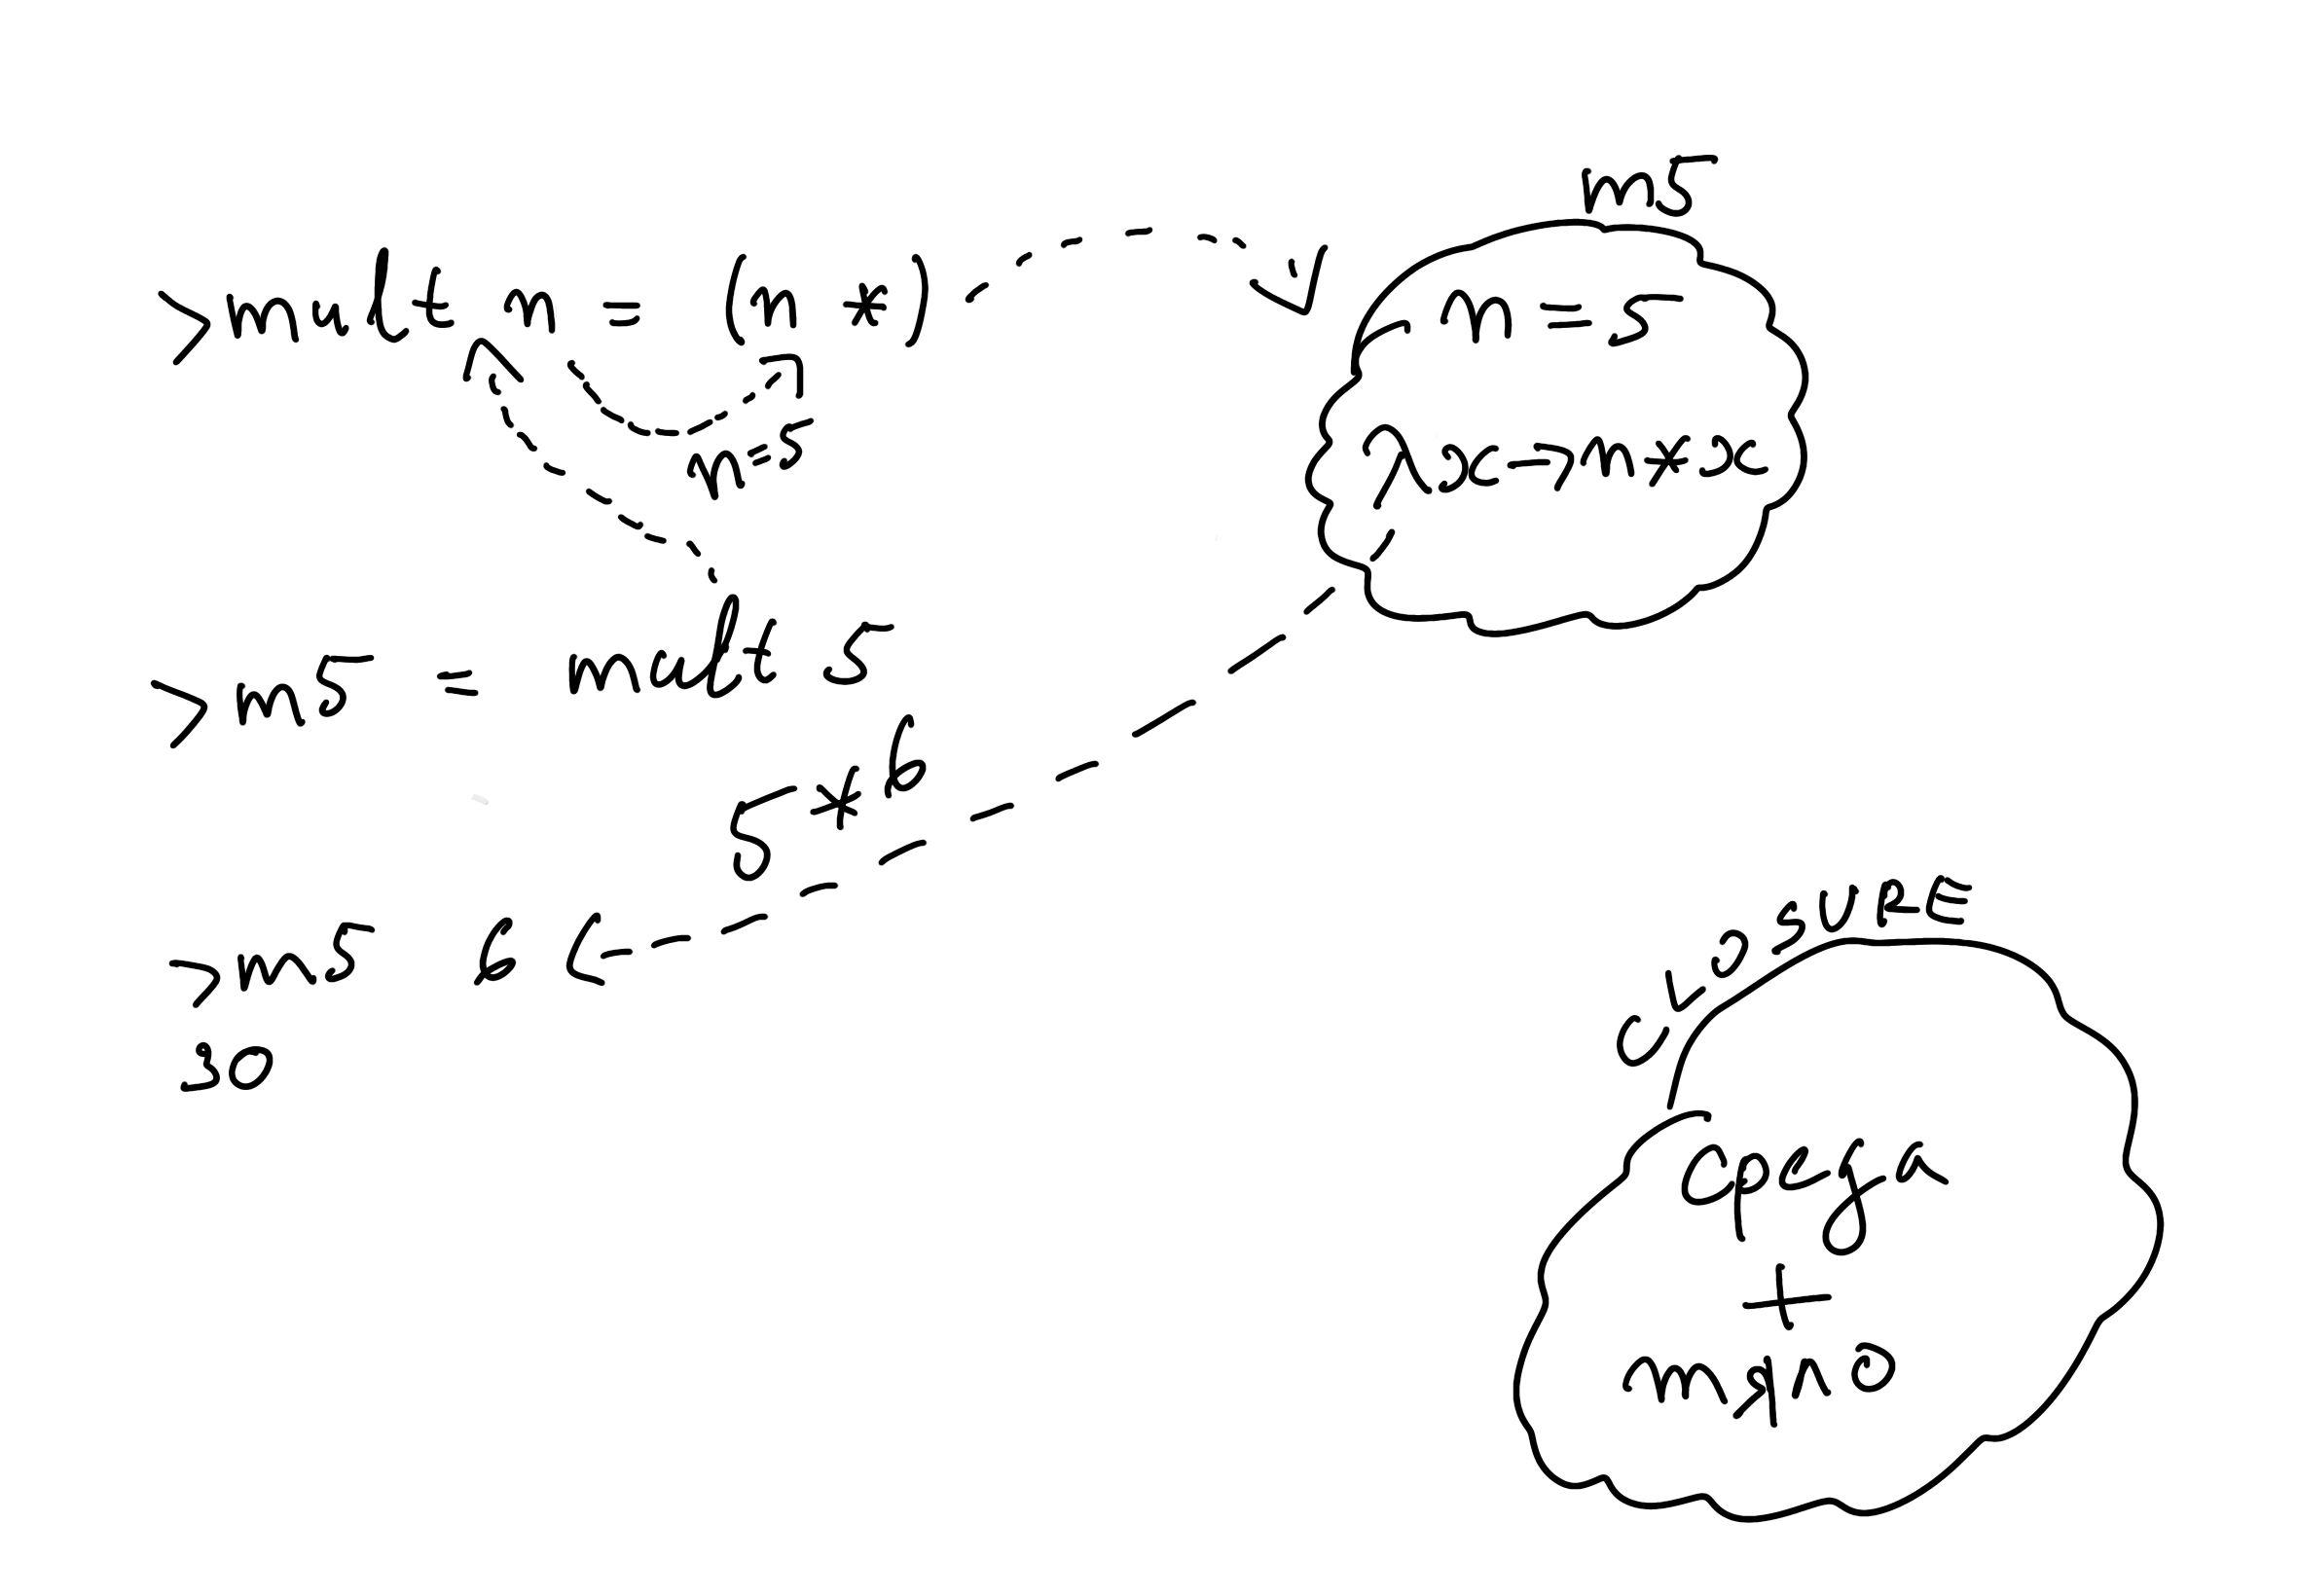
\includegraphics[width=120mm]{images/closure}};
  \end{tikzpicture}
\end{frame}


\begin{frame}[fragile]
  \frametitle{Closures}

Примери: negate, cut, switch, repeated, derive

\end{frame}


\begin{frame}
  \centerline{Благодаря за вниманието!}
\end{frame}


\end{document}


\begin{columns}[t]
  \begin{column}{0.2\textwidth}

\relscale{0.63}
\begin{lstlisting}
\end{lstlisting}
\relscale{1}

  \end{column}
  \begin{column}{0.8\textwidth}

  \end{column}
\end{columns}


